\section{软件游戏流程}

\subsection{游戏背景}
游戏名称:无敌史莱姆大冒险(Invincible Slime's Adventure)。

游戏背景:一只小史莱姆在它的旅程中经过一片极地,恰逢此时,雪霁银装素,桔高映琼枝。新奇的景色勾起史莱姆的一片玩心。而史莱姆在雪地上撒欢了一段时间后发现,它已经迷失在雪地中,在这天寒地冻的环境中,它迫切地需要收集食物并达到庇护点以存活下去。因此,史莱姆开始了它的行动……

\begin{Figure}[游戏角色设计]
    \begin{FigureSub}[史莱姆]
        \includegraphics[width=5.5cm]{build/MainCht.fig.pdf}
    \end{FigureSub}
    \hspace{2cm}
    \begin{FigureSub}[苹果]
        
\includegraphics[width=5.5cm]{build/Apple.fig.pdf}
    \end{FigureSub}
\end{Figure}

\subsection{游戏流程}

游戏发生在一个$12\times 12$的方形地图上,如\xref{fig:游戏地图示例}所示的例子。游戏的主角是一只史莱姆,其初始会出现在地图上某一指定位置。游戏的核心玩法在于两种方块,表现为蓝色的冰面和表现为白色的雪堆,史莱姆可以向上下左右四个方向沿冰面滑行,直到遇到雪堆才会停下。游戏的目标是,以最少的滑行次数,收集满散落于地图的三个苹果,到达以绿色标识的庇护所,但是,即便没有收集满三个苹果,到达庇护所也将视为过关。

游戏基于这一模式,共设立了48张地图(即48个关卡),全部关卡的地图和预设的可行解置于文档附录中。除了冰面和雪堆这两种基本方块,后续关卡中还引入六种功能各异的特殊方块,现将所有方块的功能和设定罗列如下,各方块图例如\xref{fig:游戏方块设计}所示。
\begin{Figure}[游戏地图示例]
    \begin{FigureSub}[关卡03的地图]
        \includegraphics[width=6cm]{build/Map03.fig.pdf}
    \end{FigureSub}
    \hspace{0.5cm}
    \begin{FigureSub}[关卡26的地图]
        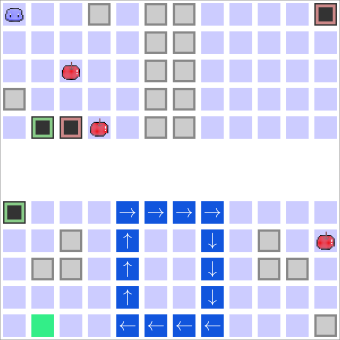
\includegraphics[width=6cm]{build/Map26.fig.pdf}
    \end{FigureSub}\\ \vspace{0.5cm}
    \begin{FigureSub}[关卡39的地图]
        \includegraphics[width=6cm]{build/Map39.fig.pdf}
    \end{FigureSub}
    \hspace{0.5cm}
    \begin{FigureSub}[关卡42的地图]
        \includegraphics[width=6cm]{build/Map42.fig.pdf}
    \end{FigureSub}
\end{Figure}

\begin{itemize}
    \item 冰面:基本方块,史莱姆在冰块上将持续滑行。
    \item 雪堆:基本方块,史莱姆将在雪堆前停下。
    \item 机关:具有四种方向,以箭头标识,史莱姆经过机关时滑行会发生转向。
    \item 碎石:类似于雪堆,但是,史莱姆撞击一次停下后将会碎裂消失变为冰面。
    \item 法阵:具有至多三对,分别以红色、绿色、蓝色标识,当史莱姆进入一个法阵时将会被传送到该组另一法阵所在方块处,并保持原有方向继续在冰面上滑行。
    \item 陷阱:冰面上的窟窿,应避开,史莱姆经过时将坠入其中,游戏失败。
    \item 闸门:具有关闭和开启两种状态,关闭时相当于雪堆,开启时相当于冰面,默认为关闭。闸门的状态由按钮控制,史莱姆每经过一次按钮,闸门状态翻转一次。
    \item 按钮:控制闸门状态,仅出现在有闸门的关卡。
    \item 庇护所:游戏终点,具有黏附性,即滑过终点时史莱姆会自动停下,游戏过关。
\end{itemize}
\begin{Figure}[游戏方块设计]
    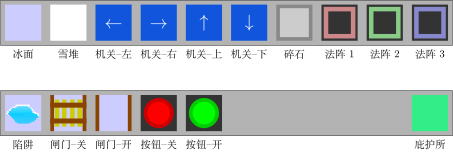
\includegraphics[width=0.95\linewidth]{build/Block.fig.pdf}
\end{Figure}

游戏具有三种可能的结束方式:若到达庇护所,游戏过关,这种情况下,苹果越多越好,步数越少越好;若到达陷阱,游戏失败;若陷入死局,即无论采取何种移动方式都无法到达庇护所,也是失败的,此时玩家需自行退出游戏界面,重新进入关卡。

\subsection{游戏界面}
游戏中主要有四个界面:启动界面、菜单界面、游戏界面、结算界面。启动界面即游戏机启动后显示的界面,也是系统的主界面,其会显示游戏名称“Invincible Slime's Adventure”并播放启动界面动画和背景音乐。按键即可进入菜单界面,菜单界面可以选择关卡,进入游戏界面。游戏界面的右侧将显示地图,游戏界面的左侧则将会显示当前关卡、已走步数、已收集的苹果数量。游戏结束后,将进入结算界面,显示所用步数和收集到的苹果总数,根据结束方式显示“YOU WIN”或“YOU FAIL”的字样,并相应播放“欢乐颂”和“致爱丽丝”的片段作为背景音乐,按键可以返回菜单界面。



\subsection{游戏操作}
游戏的操作主要包含六项:左L、右R、上U、下D,确认C、退出E。游戏中的交互同时支持三种方式:矩阵键盘、手柄摇杆、手柄体感控制。矩阵键盘键位如\xref{fig:键盘操作}所示。使用WII Nunchunk手柄时,按住C键即为确认,按住Z键即为退出,拨动手柄摇杆左右上下给出相应方向键。但特别的,在游戏界面下,按住Z键时将变为开启体感控制,此时可通过左倾、右倾、前倾、后倾手柄的方式给出左右上下的方向键。

\begin{Figure}[键盘操作]
    \includegraphics{build/Section03_01.fig.pdf}
\end{Figure}



\subsection{游戏体验}
游戏完成后,作为项目组的成员首先进行了试玩,从我们自身感受而言,即便作为游戏关卡的设计者和开发者,我们仍然能感受到相当的趣味。这表明,复赛期间重新开发的“无敌史莱姆大冒险”不仅仅再是一个功能验证,而是确实具有可玩性的游戏。
% 0
% 在每一关游戏开始时,史莱姆会从固定出发点出发,它可以在冰面上沿着一个方向直线滑行,直到其遇到其他方块。史莱姆的目标是进入到木屋躲避严寒,在这个基础上,史莱姆还会收集尽可能多的食物以抵御严寒。

% \subsection{软硬件功能划分}
% 系统的软硬件功能划分如下:硬件部分负责实现诸如显示编码、数码管扫描、蜂鸣器驱动等对速度要求较高,需要复杂时序控制的部分。硬件部分将外设封装为若干寄存器,使得软件部分不需要关心驱动外设所需的时序,而是可以直接通过寄存器操作外设的工作状态。软件部分负责游戏功能的实现,根据输入和游戏逻辑控制图像和声音。

% \subsection{软件架构}
% 软件部分主要可以分为两部分:硬件抽象层和软件逻辑层。

% 硬件抽象层将硬件部分封装的寄存器转换为C语言可用的对象。具体而言,对于每个外设,硬件抽象层会创建一个与外设寄存器排列顺序一致的结构体,随后,硬件抽象层会将外设寄存器所在内存地址强制转换为一个结构体指针,后续编程中就可用通过这个指针操作相应的外设寄存器了。硬件抽象层还会定义一些函数,例如显示部分的图形绘制函数,以及串口通讯部分的读写函数,使软硬件的交互变得更为便利。

% 软件逻辑层即实现具体游戏逻辑的部分。对于游戏中的每个界面,都会定义一个函数实现界面中的相关功能。在main函数中会调用相应界面的函数,当界面需要切换时,当前界面的函数会返回需要切换界面的编号至main函数,而main函数则会根据这一返回值确定接下来应调用哪一界面的函数。以此实现游戏多个界面间的切换和解耦。

% \subsection{软件部分的游戏流程}
% 游戏部分目前包含两个界面:游戏初始界面、游戏界面。

% 游戏内容:
% 玩家通过控制方块进行左右移动以通过正确的区域。别踩黑线!
% \begin{enumerate}
%     \item 在游戏初始界面时,会播放背景音乐,点击任意按键即开始游戏。
%     \item 在进入游戏界面后,显示屏中中会出现一个方块,显示屏下方一条中间有开口的黑线。其中方块为玩家所控制对象,黑线为方块不可通过区域,黑线开口处为方块的可通过区域。同时,数码管会被点亮。其中,左一的数码管的数值表示生命值,左二的数码管的数值表示关卡数,左三及左四的数码管的数值表示游戏得分。
%     \item 在开始游戏后,方块将会自动进行向下坠落,玩家需按下键盘上的指定按钮对方块进行左右移动。如果方块从黑线开口处通过,则游戏得分加5,如果方块从黑线所在处通过,则生命值减1,两种情况下会分别播放不同的音符予以提示。
%     \item 每次方块从屏幕最上方坠落到最下方的过程为一个周期。在一个周期结束后,方块将会保持上一周期所在的横向位置并再次出现在屏幕最上方,开始新的周期。
%     \item 当游戏得分到达50分时,游戏关卡升级,屏幕中将出现两条黑线及其相应的开口区域,开口区域为随机生成,玩家需控制方块从两个开口处依次通过。
%     \item 当生命值减少至0时,游戏结束,画面返回至游戏初始页面。
%     \item 再次点击任意按键时可再次进入游戏。
% \end{enumerate}

% 游戏目前仅代表一个简单的功能性测试,以检验游戏机系统可以完整运行。后续随着硬件功能的完善,游戏将会相应重新设计,细化游戏内容,丰富游戏交互体验。

